\subsection[Outil de coordination: git]{Outil de coordination: git}
\label{subsec:etatavanc:git}
L'�tat des scripts utilis�es par l'�quipe est mise � jour par un
syst�me de version utilisant git
\url{https://github.com/Romain-Ly/PRES}.

\subsection[Compilation MPTC]{Compilation MPTCP}
\label{subsec:etatavanc:mininet-mptcp}

Pour la r�alisation du projet, nous utilisons une machine virtuelle de
mininet install� ubuntu 13.04 32 bits, disponible ici :
\url{https://bitbucket.org/mininet/mininet-vm-images/downloads}.

La mise en place du noyau linux MPTCP (v0.88) dans une VM de mininet
(v2.10) est � 100~\% termin�.

Les paquets debian pour l'installation du noyau MTPCP sur une VM de
mininet est disponible :
(\url{https://www.dropbox.com/sh/y4ykck8rg6908ps/7V3lsV6Ggg}).


\subsection{Topologie}
\label{subsec:CR:topologie}

Nous utilisons principalement deux topologies (A et B).

La topologie A est inspir� du \emph{testbed} de l'article de
R. Khalili \cite{pareto2013}, voir \fig{fig:topoMPTCP:A}. Nous avons
ajout�, � cette topologie, des routeurs priv�s entre le client et le
serveur \emph{MPTCP} pour disposer d'un nombre de sous-flots sup�rieur � deux.\\

\begin{figure}[!htb]
  \begin{changemargin}{-2.0cm}{0.5cm}
    \centering
    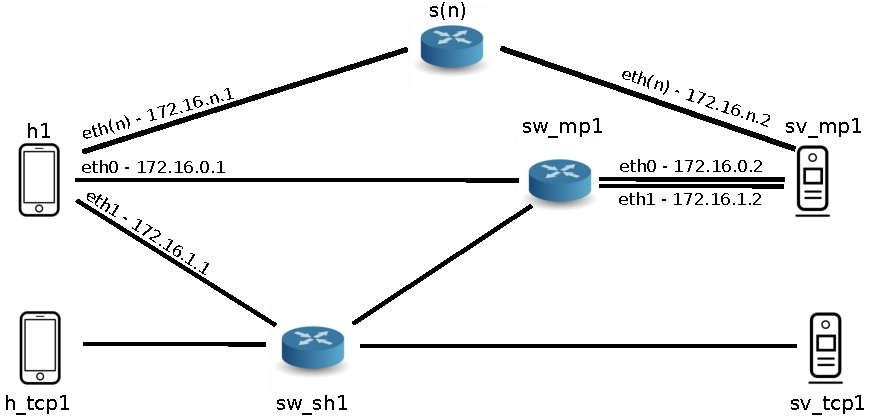
\includegraphics[width=0.7\textwidth]{../figures/mptcp_tcp/mptcp_tcp.pdf}
  \end{changemargin}
  \centering
  
  \caption{\textbf{Reproduction de la topologie de l'article de
      R. Khalili}. Le(s) \emph{switch(s)} ``S(n)'' ne sont pr�sent(s)
    que si le nombre de sous-flot est sup�rieure � deux. Pour n
    sous-flots, il y aura $n-2$ \emph{switchs} et $n-2$ liens
    suppl�mentaires. L'hyperviseur est connect� � tous les
    switchs. Pour se connecter via ssh aux h�tes, un \emph{switch} \og
    root \fg est cr�� et est connect� au \emph{switch} sw\_mp1 (non
    repr�sent� ici) voir utilisation CF linktobeadded.}
  \label{fig:topoMPTCP:A}
  
\end{figure}


La topologie B correspond au \emph{fat tree}.


\subsection{Performance de MPTCP sur mininet}
\label{sec:CR:perfMPTCP:base}

Apr�s la compilation du noyau, pour v�rifier le fonctionnement de
MPTCP nous avons mesurer le d�bit moyen en utilisant \emph{iperf} sur
la topologie A.

Les param�tres\footnote{param�tres par d�faut dans le noyau Linux}
utilis�s sont les suivants:


\vspace{1cm}
%\begin{tabular}{lp{\linewidth - 4cm}} 
\begin{tabular}{ll}
\textbf{Param�tre}& \textbf{Valeur}\\
\hline
MSS& 1460 octets\\
window size& 85,3 Koctets\\
d�lai par lien & 10 ms\\
Algorithme de congestion& LIA \cite{rfc6356}\\
\end{tabular}
\vspace{0.5cm}

Si nous fixons le MSS � 1460 octets, nous obtenons ce message
d'erreur:
\begin{verbatim}
  WARNING: attempt to set TCP maximum segment size to 1460, but got
  536
\end{verbatim}

Cependant, si nous analysons les paquets enregistr�s gr�ce � TCPdump,
nous observons que la taille maximal du MSS n�goci� pendant le
\emph{handshake} de la connexion MPTCP est de 1460 octets et que la
taille du MSS dans les paquets de donn�es est de 1428 octets.

\subsubsection{Un exemple de d�monstration}
\label{sec:CR:perfMPTCP:unique}

Ici nous allons prendre l'exemple d'une connexion avec deux sous-flots
� 100 Mbit/s. Voici la commande pour g�n�rer cet exemple:
\begin{verbatim}
sudo python ./pyMPTCP -O exp001_TC --bw 100 -t 30 -n 2 --mptcp --bwm_ng
\end{verbatim}

Pour les d�tails de l'activation de MPTCP dans le noyau et
l'utilisation des arguments des scripts python, une notice est donn�e
en Annexe 1: voir sections \ref{sec:annexe1:usepyth} page
\pageref{sec:annexe1:usepyth} et \ref{sec:annexe1:mininetParserargs}
page \pageref{sec:annexe1:mininetParserargs}.

\vspace{0.5cm}
Le d�lai (RTT) entre h1 et sv\_mp1 est de 44\,$\pm$\,11\,ms (mesur�
avec la commande ping), ce qui correspond bien au d�lai n�cessaire
pour traverser deux liens. La moyenne ici tient compte du d�lai du
premier paquet qui est envoy� vers le contr�leur qui va �tablir le
chemin vers le serveur\footnote{Il pourrait �tre n�cessaire d'enlever
  le d�lai de ce premier paquet dans une version future.}.

L'argument ``-\,-bwm-ng'' permet de lancer Bandwidth Monitor
NG\footnote{\url{http://www.gropp.org/?id=projects&sub=bwm-ng} }
(bwm-ng) et de mesurer plusieurs param�tres comme le nombre d'octets,
de paquets, le d�bit entrant ou sortant passant par chacune des
interfaces sond�es. La Figure \ref{fig:MPTCP-perfbwm-ng} montre le
d�bit entrant c�t� serveur pour ses deux interfaces, nous observons
que pour deux sous-flots aux capacit�s identiques, le d�bit mesur� est
quasi identique (une diff�rence de quelques paquets est observ�e).

\begin{figure}[htb]
    \centering
    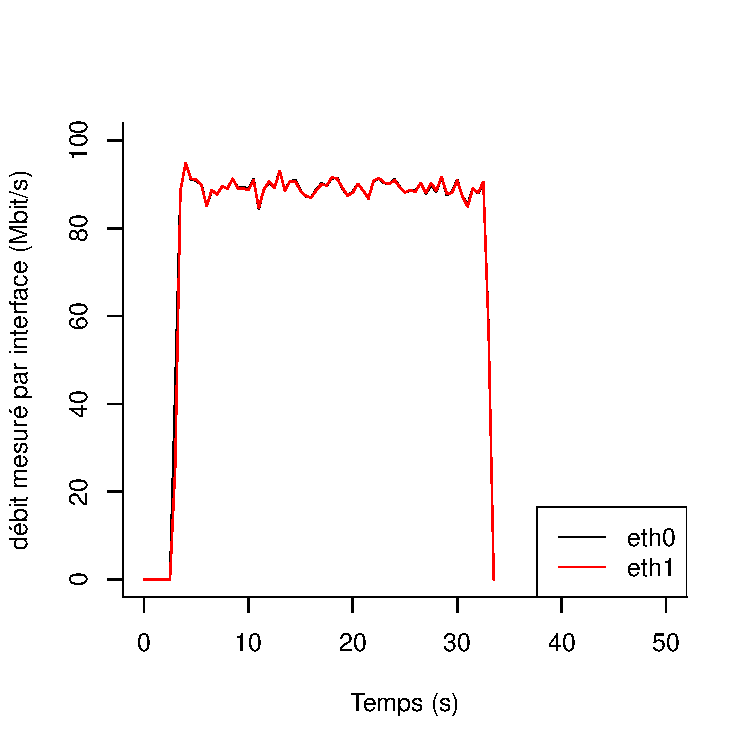
\includegraphics[width=0.7\textwidth]{../figures/bw-single.pdf}
    \caption{\textbf{D�bit entrant c�t� serveur.} �chantillonage : 2\,Hz.}
  \label{fig:MPTCP-perfbwm-ng}
\end{figure}

Pour mesurer le d�bit total g�n�r�, nous moyennons les d�bits totaux
mesur�s toutes les secondes par \emph{iperf} entre 5 secondes apr�s le
d�but de la connexion et 1 seconde avant la fin de la connexion. Nous
obtenons, c�t� serveur et pour cet exemple, un d�bit maximal de
168\,Mbit/s ce qui est attendu par les mesures de d�bit \emph{via}
bwm\_ng.


\subsubsection{Variation du d�bit maximal par lien}
\label{sec:CR:perfMPTCP:nsousflots}

Pour conna�tre les limites de la capacit� de notre simulation, nous
faisons varier le d�bit maximal par sous-flot, ainsi que le nombre de
sous-flots dans la topologie A.

\begin{figure}[htb]
    \centering
    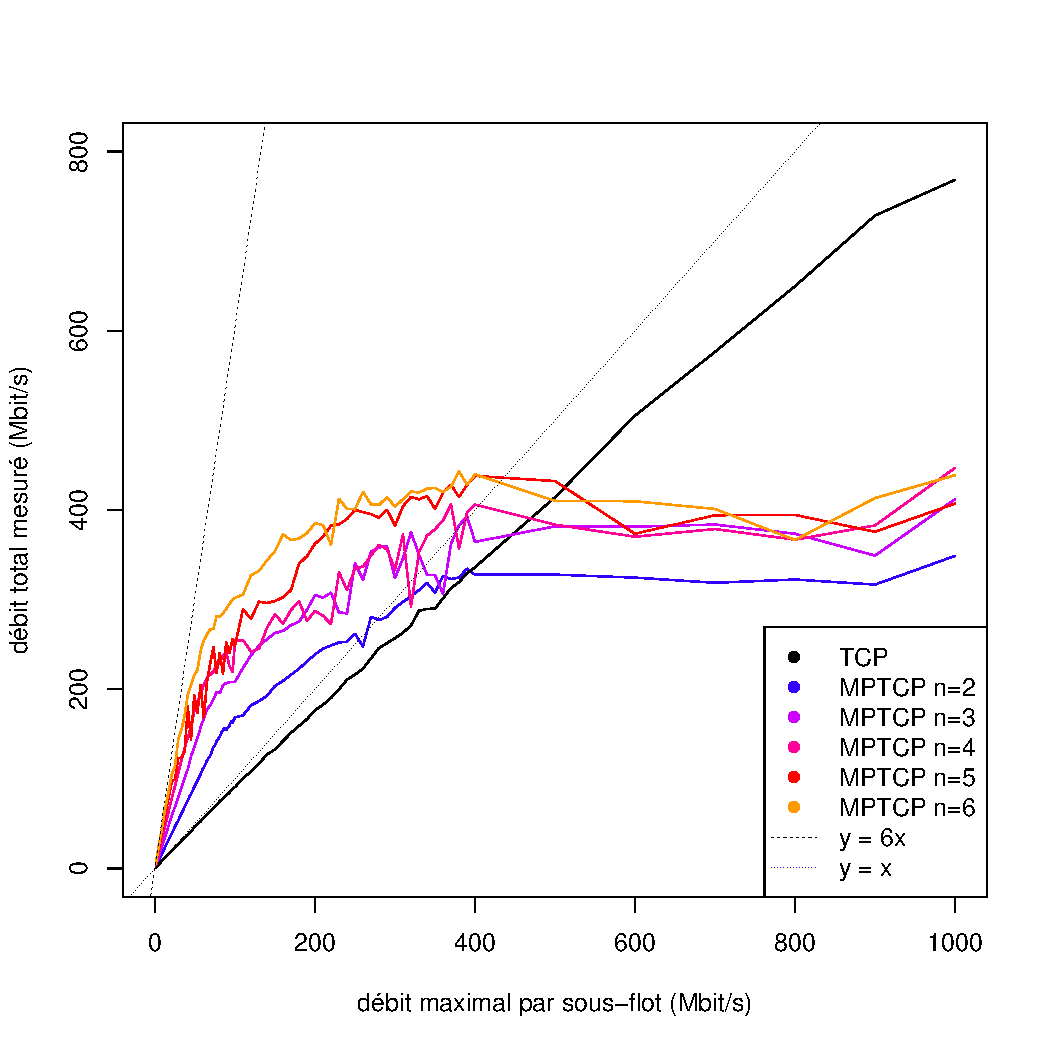
\includegraphics[width=0.7\textwidth]{../figures/bw-coupled.pdf}
    \caption{\textbf{D�bit total mesur� en fonction du d�bit maximal
        par sous-flot.} Les d�bits sont mesur�s avec \emph{iperf} pour
      une connexion TCP classique et une connexion MPTCP contenant de
      2 � 6 sous-flots.}
  \label{fig:MPTCP-perf-subflow-bw}
\end{figure}

Nous observons une phase lin�aire o� l'augmentation du d�bit par lien
ou l'augmentation du nombre de sous-flots augmente lin�airement le
d�bit total obtenu c�t� serveur. Cette phase situ�e en dessous des
100\,Mbit/s par lien correspond au but de MPTCP : augmentation du
d�bit. Cependant, les performances d�croissent rapidement et tombent
sous les performances d'une simple connexion TCP ce qui est contraire
� la nature m�me de MPTCP \cite{rfc6182}.

Ce probl�me pourrait �tre expliquer par l'utilisation non optimale de
la capacit� des sous-flots. Le \emph{bandwidth delay product} (BDP)
implique une taille minimale du tampon de r�ception. Pour un d�bit de
1000\,Mo et un RTT de 44\,ms, on obtient une taille minimale de tampon
de 5,5\,Mo. Sachant que le tampon de r�ception est partag� pour tous
les sous-flots d'une connexion MPTCP \cite{rfc6824}, la taille
minimale du tampon de r�ception doit suivre cette formule :

\begin{equation}
  \label{eq:MPTCP:buffer}
  buffer\_size \geqslant max(\{RTT_i\}_{i \in [1,n]})*\sum_{i \in [1,n]} Bandwidth_{\{i\}}
\end{equation}

C'est � dire que la taille du tampon de r�ception doit �tre le produit
du RTT maximal parmi tous les sous-flots et le d�bit total de tous les
sous-flots r�unis. Cette taille de tampon garantit l'utilisation
optimale du lien lorsque des paquets n�cessitent d'�tre retransmisent
sur des sous-flots aux d�lais lents. Dans notre simulation, il n'y a
pas de perte de paquet, la valeur minimale correspond au BDP le plus
�lev�.

Pour les m�mes propri�t�s de liens, avec deux sous-flots, nous
obtenons une taille minimale de 11\,Mo. Mininet modife automatiquement
les tampons au lancement de la topologie et les valeurs utilis�es sont
les suivantes:

\begin{verbatim}
net.core.wmem_max = 16777216
net.core.wmem_default = 163840
net.core.rmem_max = 16777216
net.core.rmem_default = 163840
net.ipv4.tcp_wmem = 10240	87380	16777216
net.ipv4.tcp_rmem = 10240	87380	16777216
net.ipv4.tcp_mem = 19326	25768	38652
\end{verbatim}

Nous observons que le tampon maximal pouvant �tre allou� par socket
est de 16\,Mo environ ce qui est largement sup�rieur � la taille
requise. De plus en augmentant la taille du tampon, nous n'observons
pas d'augmentation de performances alors qu'en le diminuant, nous
observons une diminution du d�bit mesur�
Fig. \ref{fig:mptcp:windowscale}.

\begin{figure}[!htb]
  \begin{changemargin}{-2.0cm}{0.5cm}
    \centering
    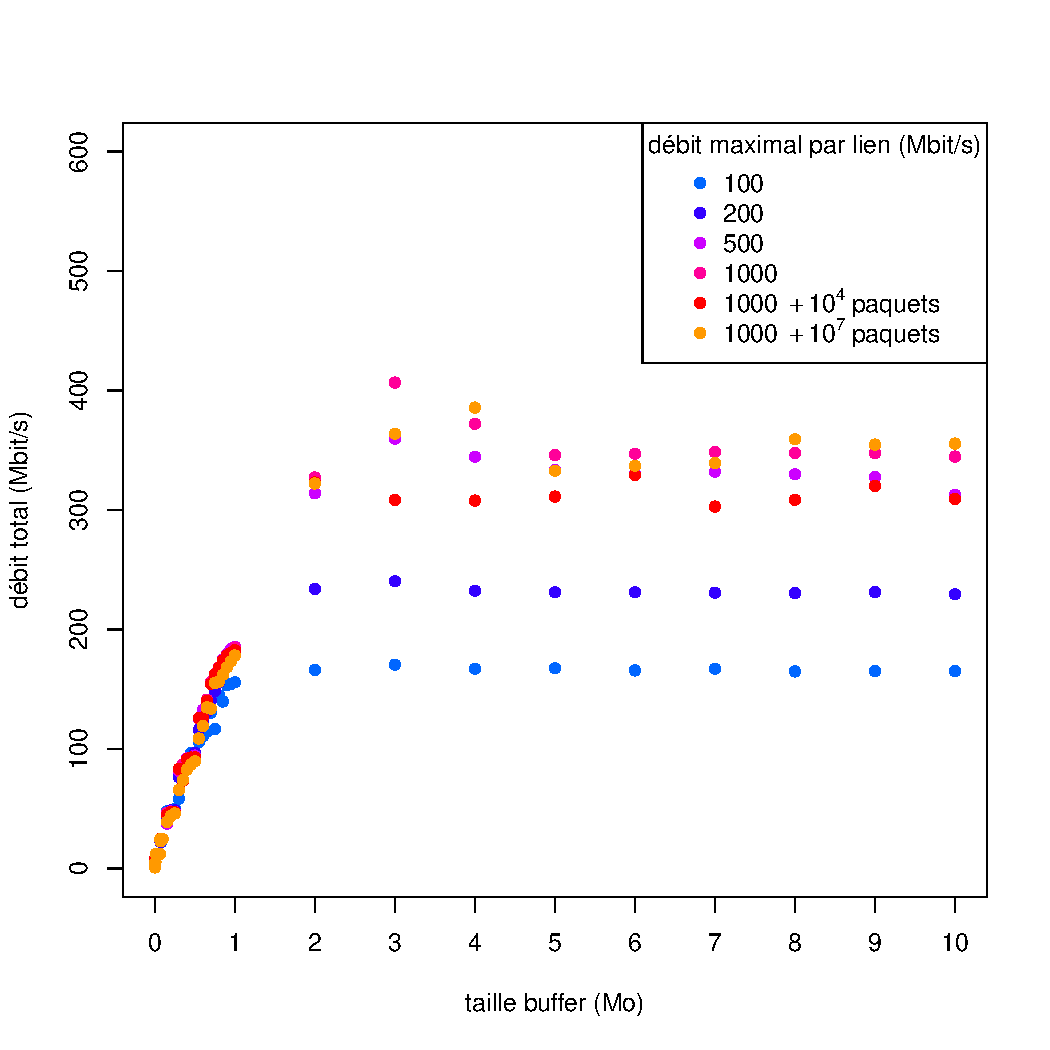
\includegraphics[width=0.7\textwidth]{../figures/ws.pdf}
  \end{changemargin}
  \centering
  
  \caption{\textbf{D�bit mesur� en fonction de la taille de la
      fen�tre}. La taille maximmale de la fen�tre TCP est modifi�e
    avec l'argument '-w' avec \emph{iperf}. La taille obtenue est
    �trangement de deux fois sup�rieure � la taille demand�. Le nombre
    de paquets correspond � la taille maximale de la queue des
    routeurs.}
  \label{fig:mptcp:windowscale}
  
\end{figure}

Nous obtenons les m�mes r�sultats en modifiant la taille maximale de
la queue des routeurs ou en modifiant les valeurs dans le noyau (voir
\ref{sec:annexe1:windowsize} page \pageref{sec:annexe1:windowsize})
que ce soit les param�tres minimum, par d�faut et maxium
d'\emph{auto-tuning} de TCP (\emph{net.ipv4}) ou les valeurs maximales
ou par d�faut pour tous les type de connexions (\emph{net.core}). Une
v�rification de la charge CPU global avec \emph{htop} ne montre pas
une saturation des processeurs (environ 15\,\% d'utilisation)
cependant, il reste � impl�menter \emph{cpuacct} pour v�rifier la
charge CPU par conteneur.


En effectuant des
recherches\footnote{\url{https://github.com/mininet/mininet/wiki/Introduction-to-Mininet\#what-are-mininets-limitations}}\footnote{\url{https://mailman.stanford.edu/pipermail/mininet-discuss/2014-January/003901.html}},
il semblerait que la limite du d�bit est li� aux n\oe uds Open vSwitch
sur Ubuntu 13.04, ce qui pour une dizaine de liens limite la capacit�
� 100 Mbit/s. C'est pourquoi, nous utiliserons des d�bits de 10 Mbit/s
environ pour les prochaines exp�riences.

